\documentclass[12pt]{article}

\usepackage[utf8]{inputenc}
\usepackage[brazil]{babel}
\usepackage[a4paper,left=3cm, right=2cm,top=2.5cm, bottom=2.5cm]{geometry}
\usepackage{amsmath}
\usepackage{graphicx}
\usepackage{float}
\usepackage{multirow}
\usepackage{authblk}
\usepackage{fancyhdr}
\usepackage{xcolor}
\usepackage{cite}


\title{\textbf{ENG1456 - Algoritmos Genéticos - Trabalho 2}}
\author{\textbf{Aluno: Matheus Carneiro Nogueira - 1810764}}
\affil{}
\author{\textbf{Professora: Karla Figueiredo}}
\affil{}
\pagestyle{fancy}
\fancyhf{}
\lhead{{\small \textcolor{gray}{PUC-Rio ENG1456}}}
\renewcommand{\headrulewidth}{0pt}
\date{}
\renewcommand{\footrulewidth}{0pt}
\fancyfoot[C]{\thepage}

\begin{document}
	\maketitle
	%\tableofcontents
	
	
\begin{abstract}
	Este documento consiste no relatório do trabalho 2 do módulo de Algoritmos Genéticos da disciplina ENG1456 da PUC-Rio. O objetivo deste trabalho é estudar diferentes modelos de Algoritmos Genéticos para a tentativa de otimização da função Rastrigin. Foi utilizada a biblioteca geneticalgorithm2 para Python. Foram consultados os materiais de aula, o livro \cite{davis1991handbook} e outros materiais devidamente referenciados. 
\end{abstract}
	
\section{Apresentação do Problema e comentários iniciais}

O objetivo é avaliar e testar todos os parâmetros do Algoritmo Genético para encontrar a função de mínimo para o problema no menor tempo possível, ou seja, com a menor quantidade de gerações. O problema a ser minimizado é a função Rastrigin, definida por:
\begin{equation*}
	f(x)=A_n+\sum_{i=1}^{n}[x_i^2-Acos(2\pi x_i)]
\end{equation*}

\begin{figure}[H]
	\centering
	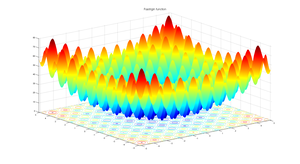
\includegraphics[width=0.7\linewidth]{Imagens/Rastrigin_function}
	\caption{Plot da função Rastrigin}
	\label{fig:rastriginfunction}
\end{figure}

Em cada seção desse relatório será variado algum parâmetro do algoritmo genético com o intuito de melhorar a minimização da função Rastrigin, com exceção da próxima seção que apresentará os resultados para os parâmetros iniciais padrões da biblioteca. Para visualizar e comparar resultados, serão fornecidas tabelas com os valores adotados para os parâmetros e imagens dos gráficos gerados pelo código.

Os parâmetros que serão variados são \textit{max\_num\_iterarion}, \textit{population\_size}, \textit{mutation\_probability}, \textit{elit\_ratio}, \textit{crossover\_probability}, \textit{parents\_portion} e \textit{crossover\_type}. Sempre será variado um parâmetro por vez, mantendo os demais iguais ao GA inicial. Isso será feito para avaliar o impacto de cada parâmetro na qualidade do GA. Ao final, será executado um GA com os melhores valores para cada parâmetro variado.

Serão sempre realizados 5 experimentos para cada configuração de GA e a análise será realizada com base nos resultamos médios de cada configuração.

\section{GA com parâmetros iniciais dados}

Os parâmetros utilizados no GA são:
\begin{table}[H]
	\centering
	\begin{tabular}{|l|l|l|l|}
		\hline
		max\_num\_iterarion    & population\_size & mutation\_probability & elit\_ratio \\ \hline
		100                   & 100               & 0.1                     & 0.01           \\ \hline
		crossover\_probability & parents\_portion & crossover\_type       &             \\ \hline
		0.5                     & 0.3                & Uniform                     &             \\ \hline
	\end{tabular}
\end{table}

\section{Variação de max\_num\_iterarion} 

Esse parâmetro define por quanto tempo nosso algoritmo ficará executando, o que, em outras palavras, significa a quantidade máxima de gerações. É importante que esse valor não seja pequeno demais para que a solução possua tempo para evoluir até uma solução razoável. Por outro lado, um valor alto pode ser desnecessário caso o algoritmo convirja para algum valor ótimo em menos gerações que o número máximo.

\begin{table}[H]
	\centering
	\begin{tabular}{|l|l|l|l|l|}
		\hline
		\multicolumn{4}{|l|}{Número máximo de gerações}& Padrão \\ \hline
		10   & 50    & 200    & 500   & 100 \\ \hline
	\end{tabular}
\end{table}

\section{Variação de population\_size}

O tamanho da população é a quantidade de indivíduos em cada geração. Podemos pensar na variação desse parâmetro como uma intensificação de busca paralela. Quanto mais indivíduos na população, maior o paralelismo da busca pela solução ótima, embora exija mais capacidade computacional. Uma população pequena demais levaria muito tempo para alcançar um valor de aptidão específico enquanto que uma população maior o alcançaria mais rápido.

\section{Variação de mutation\_probability}

Variar a taxa de mutação é variar a aleatoriedade do processo de evolução do GA, uma vez que uma mutação é uma alteração aleatória em alguns dos genes, ou indivíduos, do algoritmo. Valores de mutação muito altos geram processos muito aleatórios que podem frear a evolução da minimização, embora uma taxa pequena seja importante para aumentar as chances do algoritmo ser capaz de gerar todas as combinações de indivíduos.

A tabela abaixo exibe os diferentes valores de taxa de mutação testados:

\begin{table}[]
	\begin{tabular}{|l|l|l|l|l|}
		\hline
		\multicolumn{4}{|l|}{Taxa de Mutação} & Padrão \\ \hline
		0.001    & 0.25    & 0.5    & 0.75    & 0.1    \\ \hline
	\end{tabular}
\end{table}

\section{Variação de elit\_ratio}

Esse parâmetro configura o elitismo do algoritmo genético, sendo a taxa em si a porcentagem dos melhores indivíduos que será mantida para a próxima geração. Como sabemos, o elitismo é importante para mantermos a curva de otimização monotônica, neste caso sempre decrescente haja vista o fato do problema ser uma minimização. Uma taxa zero significa não haver elitismo. Taxas muito altas freiam o processo uma vez que haverá poucos novos indivíduos sendo gerados a cada geração. Taxas pequenas demais, por sua vez, aumentam as chances de termos mais indivíduos piores do que melhores na próxima geração.

A tabela abaixo exibe os diferentes valores de taxa de elitismo testados:

\section{Variação de crossover\_probability}

Variar a taxa de crossover significa variar a taxa com a qual o algoritmo gera novos descendentes a partir dos progenitores. Altas taxas de crossover aumentam a combinação de progenitores para a geração de filhos, enquanto baixas taxas fazem com que mais filhos sejam idênticos aos pais. Taxas altas demais não são interessantes por "embaralhar" demais os filhos, fazendo com que o perfil da evolução possa ser perdido. Por outro lado, taxas pequenas demais também não são interessantes por diminuir a variabilidade genética dos filhos, o que pode frear a evolução.

A tabela abaixo exibe os diferentes valores de taxa de crossover testados:

\begin{table}[H]
	\centering
	\begin{tabular}{|l|l|l|l|l|}
		\hline
		\multicolumn{4}{|l|}{Taxa de Crossover} & Padrão \\ \hline
		0    & 0.25    & 0.75    & 1   &0.5 \\ \hline
	\end{tabular}
\end{table}

\section{Variação de parents\_portion}

\textbf{DUVIDA: ISSO AQUI TA MUITO PARECIDO COM ELITISMO}

\section{Variação de crossover\_type}

São três os tipos de crossover disponíveis: um ponto, dois pontos e uniforme. Enquanto os dois primeiros simplesmente escolhem, aleatoriamente, um ou dois pontos de corte do gene para cruzamento, o último utiliza um padrão, também aleatório, para comparar com os progenitores. Os dois últimos tipos, dois pontos e uniforme, são capazes de combinar todos os padrões dos progenitores, enquanto o de um ponto não.

\begin{table}[H]
	\centering
	\begin{tabular}{|l|l|l|}
		\hline
		\multicolumn{2}{|l|}{Tipos de Crossover}&Padrão \\ \hline
		OnePoint    & TwoPoints    & Uniform    \\ \hline
	\end{tabular}
\end{table}
	
	\bibliography{bibliografia} 
	\bibliographystyle{plain}
\end{document}